\documentclass[a4paper, 12pt, titlepage]{article}

% Including needed packages
\usepackage[margin=2cm]{geometry}
\usepackage{amsmath}
\usepackage{graphicx}
\usepackage{subfig}
\usepackage{float}
\usepackage{hyperref}

\title
{{\em Machine learning 2}\\
Exercise sheet 2}
\author{FLEISCHMANN Kay, Matrnr: 352247\\
	ROHRMANN Till, Matrnr: 343756}
\date{\today}

\begin{document}

\maketitle

\section{Swissroll}

\begin{figure}[H]
	\centering
	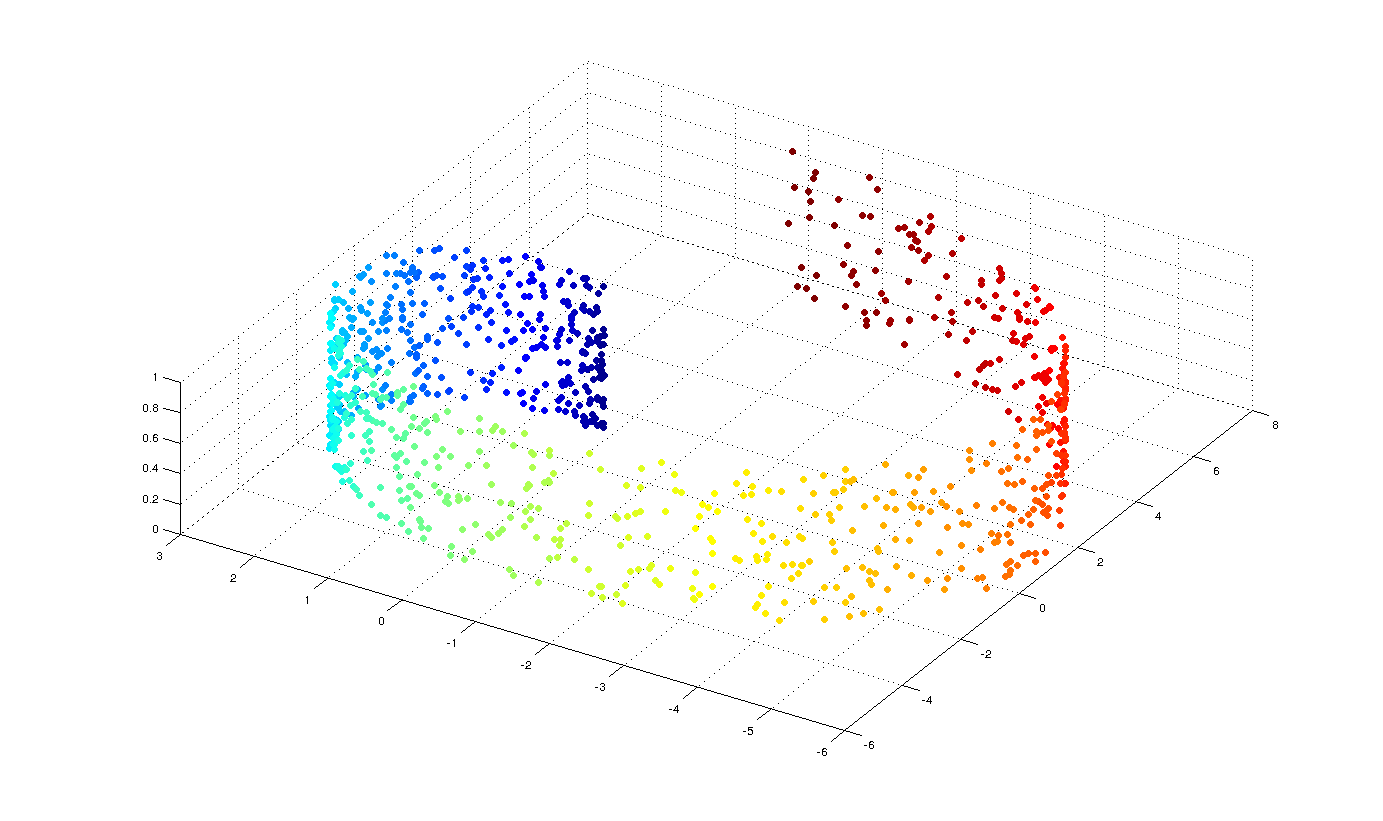
\includegraphics[width=17cm]{images/swissroll.png}
	\caption{Generated swissroll data.}
\end{figure}

\begin{figure}[H]
	\centering
	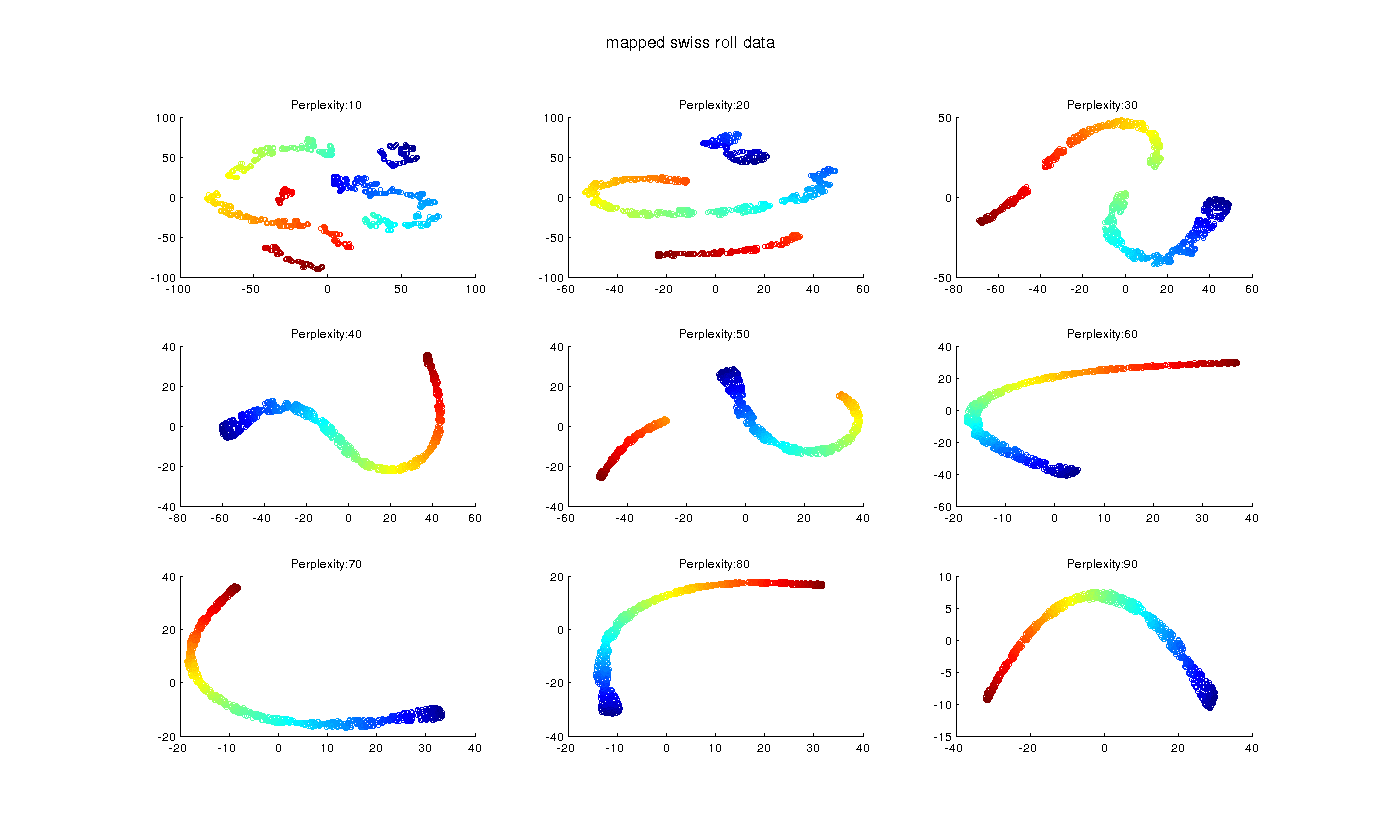
\includegraphics[width=17cm]{images/swissrollMapped.png}
	\caption{T-SNE embedding of swissroll data for different perplexity values.}
\end{figure}

We can observe that the T-SNE method did not find a good candidate for the true embedding.
The higher the perpelxity the more connected is the found mapping.
Even with a high value for perplexity the found mapping is still slightly curved.
The authors of T-SNE admit as well that the algorithm cannot really find the true embedding of a swissroll and propose to use a more lightly-tailed t-distribution for better results.
Let us finish with a quote from the authors:
\begin{quotation}
	''But frankly... who cares about Swiss rolls when you can embed complex real-world data nicely?'', \url{http://homepage.tudelft.nl/19j49/t-SNE.html}
\end{quotation}

\section{Show MNIST}

\begin{figure}[H]
	\centering
	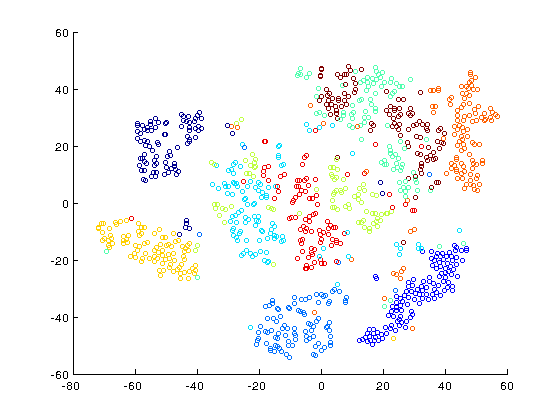
\includegraphics[width=17cm]{images/MNIST_points_only.png}
	\caption{2-dimensional embedding of the MNIST data found by the T-SNE algorithm.}
\end{figure}

\begin{figure}[H]
	\centering
	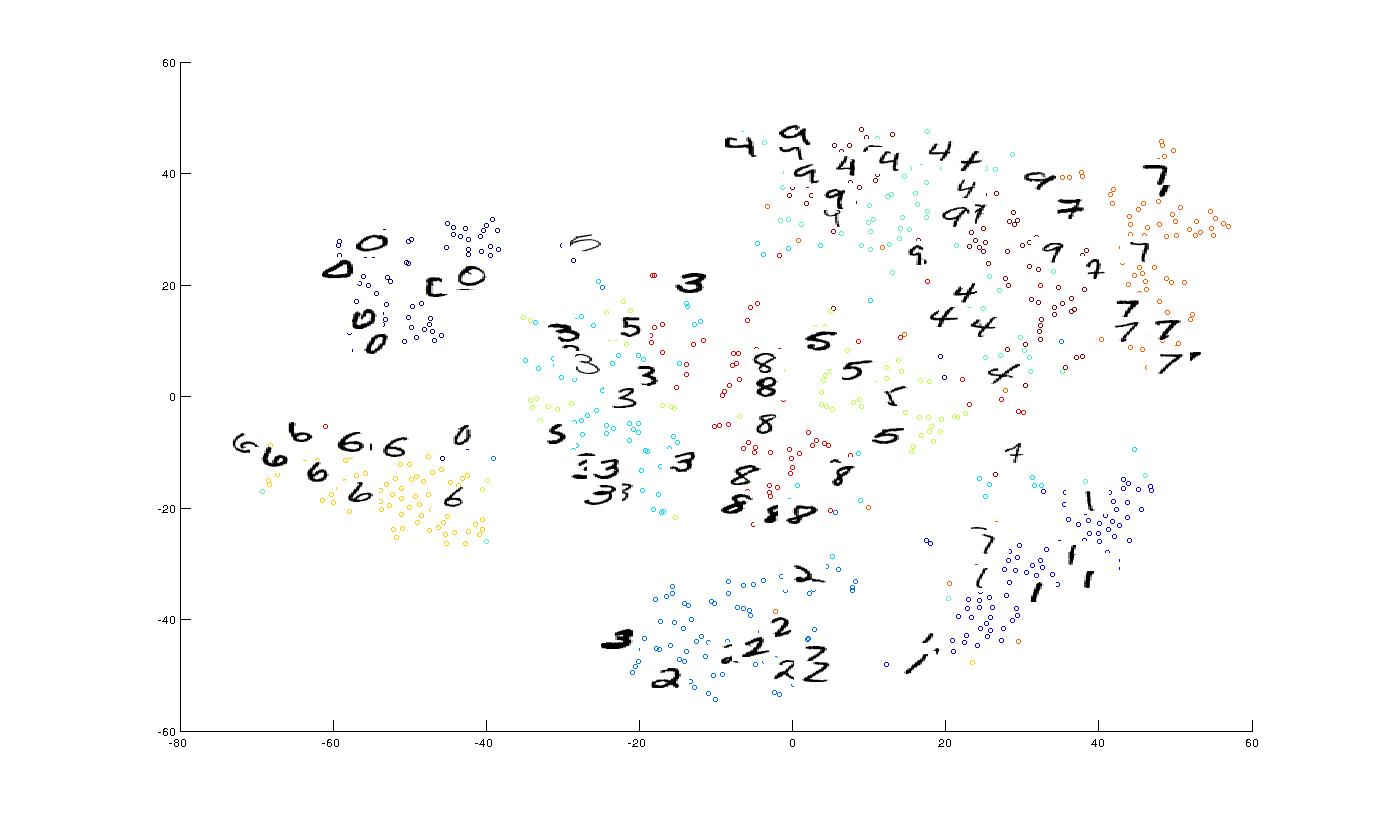
\includegraphics[width=17cm]{images/MNIST.png}
	\caption{2-dimensional embedding of the MNIST data found by the T-SNE algorithm with digit annotation.}
\end{figure}

\end{document}
